\chapter{Introduction}
\label{ch1_introduction}
\section{Motivation}

Technology scaling has led to implementation of larger circuits on a single chip. At the same time, the saturation of frequency scaling has led to exploration of parallelism by running multiple applications on hardware to gain speedup. These days both software and hardware solutions e.g. Desktops, Laptops, General Purpose Processors are supplied with multiple processors or hardware accelerators which consist of multiple small execution units to facilitate parallelism for reducing the computation time of applications. 

\vspace{0.25cm}
 Various hardware accelerators are based on GPU's, Cell Processors or FPGA's. At times software execution of certain applications takes more time than the hardware execution. Depending on the algorithm,specific accelerators may perform better than other accelerators. Hence running an algorithm efficiently is ideally a mapping an algorithm to architecture problem.
\begin{figure}[!h]
\centering
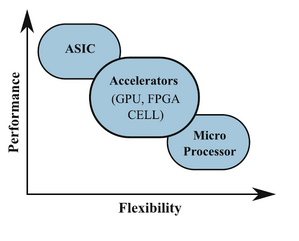
\includegraphics[scale=0.65]{figures/performance.png}
\caption{Performance Vs. Flexibility for Different Architectures.(Source \ref{architechture})}
\label{fig:Performance}
\end{figure}
\vspace{0.25cm}
 However there are certain trade-offs that need to be taken into account. e.g as given in figure \ref{fig:Performance} ASIC give the best performance in terms of time and power, but it offers less flexibility. On the other hand Microprocessors offer flexibility for programming while compromising on performance. FPGA offer hardware reconfigurablility, so it is preferred for customized designs.

\vspace{0.25cm}
 Most of the applications in present environment are computation intensive and require real time processing.For such applications performance can be enhanced by using hardware software co-design, wherein a part of an algorithm can be offloaded to hardware accelerator, with the help of bus architectures. The challenge in this process is to identify the portions of the applications which will give speedup on hardware under resource constraints. Usually the identification is based on the execution times or computation requirements.  
\begin{figure}[!h]
\centering
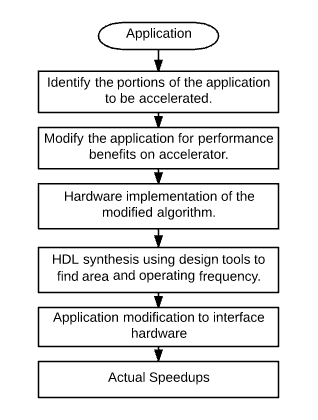
\includegraphics[scale=0.65]{figures/DSE.png}
\caption{Design Space Exploration for Algorithm Acceleration.(Source \ref{architechture})}
\label{fig:DSE}
\end{figure}
\vspace{0.25cm}

 When hardware accelerators are used, certain modifications specific to the accelerator help in getting performance benefits. e.g. in FPGA, datatypes and bit widths have significant impact on the performance. e.g. Single precision floating point datatype consumes lesser number of resources than double precision floating point datatype. Similarly fixed point computation units require lesser number of resources than floating point computation units, which can be used to increase number of concurrent executions of an algorithm and hence increasing in parallelism which may help to gain speedup. However these modifications directly impact the correctness of the algorithm. 
 
\vspace{0.25cm}
In this report, the first two steps of the design space exploration for algorithm acceleration as given in figure \ref{fig:DSE} are explored for two algorithms:FHEW and Deep Neural Network. The focus is on identification of compute intensive portions of the algorithm to be accelerated on hardware by thoroughly studying the functionality and the modification of underlying arithmetic for performance benefits. Implementation of compute intensive portion for HDL, and the gain estimation in terms of area and latency is also studied using the tool Vivado HLS.


\section{Contribution}
The main contributions can be summarized as follows:

\vspace{0.25cm}
\textbf{Fully Homomorphic Encryption (FHEW) Algorithm}
\begin{itemize}
\item
Understanding the algorithm and the existing implementation to identify the computation intensive modules of the algorithm. 
\item
Experiments of modifications of the existing library from double precision float to single precision float.
\item
Bottom-up analysis of Fast Fourier Transform, starting from a single butterfly unit, to yield a resource optimized implementation of 1024-point FFT, for efficient implementation of FHEW on hardware.
\end{itemize}

\textbf{Deep Neural Network}
\begin{itemize}
\item
Understanding the fixed point arithmetic and writing C scripts to implement fixed point mathematics.
\item
Modification of the existing implementation to support fixed point arithmetic.
\item
Analyzing the inaccuracy that can be tolerated in the algorithm, by varying the number of bits used for fixed point Q format. 
\item
Estimating the improvement in area and latency by implementing the computation intensive module for hardware using Vivado HLS. 
\end{itemize}

\section{Organization}

The remainder of the report is organized as follows:

\vspace{0.25cm}
Chapter \ref{Chapter2} gives background information on Fully Homomorphic Encryption Algorithm(FHEW), Deep Neural Network and Basics of floating point and fixed point arithmetic.\par
\vspace{0.25cm}
Chapter \ref{Chapter3} presents the modification of arithmetic of FHEW from double precision floating point to single precision floating point and a thorough analysis of the results.\par
\vspace{0.25cm}
Chapter \ref{Chapter4} discusses the implementation of an area optimized 1024 point FFT (Fast Fourier Transform) on Vivado HLS,starting from the analysis of smallest butterfly compute unit.\par
\vspace{0.25cm}
Chapter \ref{Chapter5}, discusses the existing implementation of lenet model for classification of MNIST dataset.It also discusses the mathematics of fixed point briefly and a library \textit{Libfi} which is used to integrate fixed point mathematics with the above mentioned implementation of Lenet model. It also tabulates the results of the modification on accuracy, area and latency.  \par
\vspace{0.25cm}
Chapter \ref{Chapter6} summarizes the results of the analysis and suggests areas for future work.







